\documentclass[11pt,a4paper]{report}

% Aberstwyth dissertation LaTeX Template
% Authors: Dr. Hannah Dee (hmd1@aber.ac.uk), Neil Taylor (nst@aber.ac.uk)
% This has been adapted from the Leeds Thesis template and the 
% Group Project template for Computer Science in Aberystywth University.
% 
% All comments and suggestions welcome.
%
% Template designed to be used with pdflatex: it may need alteration to
% run with a different LaTeX engine.
%
% Note - this is offered as a starting point for your work. You are not 
% required to use this template and can choose to create your own document 
% without it. 

% To build document on the unix command line, run four commands:
 
% pdflatex dissertation
% bibtex dissertation
% pdflatex dissertation
% pdflatex dissertation

% you will end up with dissertation.pdf 
\usepackage{mmp}

\usepackage{graphicx}
\graphicspath{{Images/}}

% the following packages are used for citations - You only need to include one. 
%
% Use the cite package if you are using the numeric style (e.g. IEEEannot). 
% Use the natbib package if you are using the author-date style (e.g. authordate2annot). 
% Only use one of these and comment out the other one. 
\usepackage{cite}
%\usepackage{natbib}

% Use the following to selectively exclude chapters
%\includeonly{cover,abstract,acknowledge,declare,chapter1,chapter2}

\begin{document}
\setlength{\parindent}{0in}
\setlength{\parskip}{.1in}
% all of the include directives below refer to tex files
% so 
\title{Hansard Historical Sentiment Analysis and Comparison}

% Your name
\author{Adam Neaves}

% Your email 
\authoremail{adn2@aber.ac.uk}

\degreeschemecode{GH7P} %e.g. G400 
\degreeschemetitle{Artificial Intelligence and Robotics} % e.g. Computer Science
\degreetype{BSc}

\modulecode{CS39440} % i.e. CS39440, CC39440, CS39620
\moduletitle{Major Project} % i.e. Major Project or Minor Project

\date{4th March 2018} % i.e. the date of this version of the report

\status{Draft} % Use draft until you create the release version. Then, change this to Release.
\version{1.1}

%The title and name of your supervisor.
\supervisor{Dr. Amanda Clare} 

%The email for your supervisor. 
\supervisoremail{afc@aber.ac.uk}

\maketitle

 includes cover.tex - to change the content,
% edit the tex file

\pagenumbering{roman}

% This is the front page

\title{Hansard Historical Sentiment Analysis and Comparison}

% Your name
\author{Adam Neaves}

% Your email 
\authoremail{adn2@aber.ac.uk}

\degreeschemecode{GH7P} %e.g. G400 
\degreeschemetitle{Artificial Intelligence and Robotics} % e.g. Computer Science
\degreetype{BSc}

\modulecode{CS39440} % i.e. CS39440, CC39440, CS39620
\moduletitle{Major Project} % i.e. Major Project or Minor Project

\date{4th March 2018} % i.e. the date of this version of the report

\status{Draft} % Use draft until you create the release version. Then, change this to Release.
\version{1.1}

%The title and name of your supervisor.
\supervisor{Dr. Amanda Clare} 

%The email for your supervisor. 
\supervisoremail{afc@aber.ac.uk}

\maketitle

                        

% Set up page numbering
\pagestyle{empty}

% declarations of originality 
\thispagestyle{empty}

%%%
%%% You must sign the declaration of originality. 
%%%
%%% You are submitting this electronically. Therefore, to sign, you 
%%% type your name and date to replace the .... characters. 
%%%
\begin{center}
    {\LARGE\bf Declaration of originality}
\end{center}

I confirm that:

\begin{itemize}
\item{This submission is my own work, except where 
clearly indicated.}

\item{I understand that there are severe penalties for Unacceptable Academic Practice, which can lead to loss of marks or even the withholding of a degree.}
 
\item{I have read the regulations on Unacceptable Academic Practice from the University's Academic Quality and Records Office (AQRO) and the relevant sections of the current Student Handbook of the Department of Computer Science.}
 
\item{In submitting this work I understand and agree to abide by the University's regulations governing these issues.}
\end{itemize}

\vspace{2em}
Name ............................................................  \\

\vspace{1em}
Date ............................................................ \\

%%% 
%%% We would like to make a selection of final reports available to students that take 
%%% this module in future years. To enable us to do this, we require your consent. You 
%%% are not required that you do this, but if you do give your consent, then we will have 
%%% the option to select yours as one of a number of reports as examples for other 
%%% students. If you would like to give your consent, then please include the following 
%%% text and type your name and date to replace the .... characters. 
%%% 
%%% If you do not wish to give your consent, please remove this from your report. 
%%%
\vspace{1em}
\begin{center}
    {\LARGE\bf Consent to share this work}
\end{center}

By including my name below, I hereby agree to this dissertation being made available to other students and academic staff of the Aberystwyth Computer Science Department.  

\vspace{2em}
Name ............................................................  \\

\vspace{1em}
Date ............................................................ \\
               

\thispagestyle{empty}

\begin{center}
    {\LARGE\bf Acknowledgements}
\end{center}

I would like to express my thanks to Amanda Clare, my supervisor on this project, without whose guidance I would've gotten lost in the details.

I would also like to thank Tom Doyle, my friend, roommate, and fellow Comp Sci student for being a good listener when i needed to talk through a problem. He was the best rubber duck a programmer could ask for.

I'm grateful to my mother and sister for their support during my career as a student. Without their pushing I could never have achieved as much as I have.

Finally, I'd like to thank my partner, River. Without their patience I would not have known how to deal with the stress, and whose support was invaluable despite often not knowing what I was talking about. % Acknowledgements
\thispagestyle{empty}

\begin{center}
    {\LARGE\bf Abstract}
\end{center}

Include an abstract for your project. This should be no more than 300 words.                 % Abstract

\pagenumbering{roman}
\pagestyle{fancy}
\fancyhead{}
\fancyfoot[C]{\thepage}
\renewcommand{\headrulewidth}{0 pt}
\renewcommand{\chaptermark}[1]{\markboth{#1}{}}

\tableofcontents   
\newpage
\listoffigures
\newpage 
\listoftables
\newpage

% Set up page numbering
\pagenumbering{arabic}

\setchapterheaderfooter

% include the chapters
\chapter{Background \& Objectives}

\section{Background}
\label{sec:bck_background}
\subsection{Hansard Dataset}
\label{sec:bck_hansard}
The Hansard is a set of documents produced by the British Parliament, which began in the 18th and 19th century. These documents contain reports and details of debates in the House of Commons, going back to the year 1803. Eventually, in 1907, these reports were made official and started being produced by Parliament itself, becoming “The Official Report”, though still unofficially known as Hansard. Along with becoming official, a report was officially defined as being one:
\begin{quote} “which, though not strictly verbatim, is substantially the verbatim report, with repetitions and redundancies omitted and with obvious mistakes corrected, but which on the other hand leaves out nothing that adds to the meaning of the speech or illustrates the argument"\cite{HouseofCommonsInformationOffice2010}
\end{quote}
Hansard is available in a variety of versions. The most commonly used and best known version is the Daily Hansard, which appears each morning and reports the previous day’s proceedings. However, access to this is via an API that only provides the most recent 7 days. For this project, most training and processing will be done on the Historical Hansard dataset, which is a dataset containing all 6 series of Hansard, between 1803 to 2004, though it is expected that some of the older documents will be less useful for this project due to the likelihood of them using outdated speech that would no longer be relevant.

The Historical Hansard Dataset is available online in an XML format. Multiple documents per series are available, each document covering a few days debates at most. It is a large dataset, reaching around 10Gb in size in total. Most of the documents available are scanned from hard copies, rather than typed up directly, meaning there is a possibility of small errors from the scanning process that may have to be dealt with. Additionally, from preliminary investigation, the data itself appears to be only loosely formatted, and each of the six series appear to be formatted in a slightly different way, so any system designed to read this data will have to be capable of dealing with any changes to formatting.

\subsection{Natural Language Processing}
\label{sec:bck_NLP}
Natural Language Processing (NLP) is the exploration of how computers can be used to understand and manipulate natural language text or speech to do useful things\cite{chowdhury2003natural}. Computers are very good at dealing with numbers and performing complex calculations at high speed, but they are not as good at understand spoken or written language. Because of this, a large part of NLP is the act of processing the data, or text, to make it easier for the computer to understand and work with, as well as gathering knowledge on how human beings understand and use language so that appropriate tools and techniques can be developed\cite{chowdhury2003natural}. NLP covers multiple topics, such as \emph{Named Entity Recognition}, \emph{Part of Speech Tagging}, and \emph{Sentence Boundary Disambiguation}. However, the part this project is mainly interested is the act of \emph{Sentiment Analysis}.

Sentiment Analysis, also known as Opinion Mining, is the process of identifying and extracting the opinions expressed in a piece of text\cite{Liu2010}. It aims to determine the attitude of a speaker or writer towards a topic, or the overall polarity of a piece of text. This can be a judgment made by the writer or speaker, in the case of reviews, or the emotional state of the speaker or writer.

A basic version of Sentiment Analysis classifies the polarity of a piece of text, classifying it as either positive, negative or neutral. A more advanced version would be, for example, looking at emotions expressed in the text, classifying it as angry, happy, or sad, as some examples. A basic method used can be to compare a piece to two lists of words, one a list of words that usually denote a positive polarity, and one that usually denotes a negative polarity. A system can then simply count the number of positive and negative words in a piece of text, account for any negation (Saying \emph{not great} would change the word \emph{great} from a positive to a negative word, for instance) and whichever type of word was most common would denote the piece of text’s sentiment. However, this method is likely only useful for those pieces of text where it’s known that strong sentiment is likely to be expressed in a simple enough manner, in text such as a review of a product or film.

Stance Detection is another aspect of Natural Language Processing, similar to Sentiment Analysis. However, the difference here is that Stance Detection sets out to classify the stance of text towards a particular target, or entity. Whereas Sentiment Analysis is the overall mood or polarity of text, Stance Detection specifically looks to see if the text is for, against, or neutral towards something\cite{Augenstein2016}. An example would be detecting the stance of a news article towards the subject it's being written about. This may be more applicable to the Hansard Dataset than Sentiment Analysis as the members of parliament are likely to be expressing some form of stance on a topic that they are debating, but also somewhat more complicated to do, as the subject of the stance must also be discovered from the text, which is not guaranteed to be explicitly stated.

\subsection{Related Work}
\label{sec:bck_related}

In researching the potential design of project, a few relevant pieces of work done by others were discovered, some of which had a useful impact on the design of this project. 

\subsubsection{Towards Sentiment Analysis on Parliamentary Debates in Hansard}
\emph{Towards sentiment analysis on parliamentary debates in Hansard}\cite{Onyimadu2014} is a paper which discussed the progress made by \textbf{Onyimadu \emph{et al}} towards applying classic sentiment analysis techniques to the Hansard dataset, such as word association. The paper details the proposed approach to sentiment analysis, by using \emph{“…heuristic classifiers based on the use of statistical and syntactic clues in the text…”} and using a sentiment lexicon base known as the MPQA corpus (Multi Perspective Question Answering) to identify sentences containing known positive or negative words. They first classify a sentence using this lexicon, annotating sentences as possitve or negative depending on the number of positive or negative words, before then applying syntactic clues to improve the classification, such as the presence of negations, such as \emph{“not”} or \emph{“never”}, and the inclusion of intensifying adverbs such as \emph{“very”}. The paper reports an average of 43\% correctly annotated sentences, claiming that the correctly annotated sentences were those \emph{“…without compound opinions, sarcasm and comparative sentences…”,} showing that the style of debate speech renders their syntactic and lexical based approach insufficient for the task.

This paper demonstrates the need to customize sentiment analysis for the Hansard Dataset, as it shows that the standard techniques used are not applicable to the debate speech. Any design for the project should therefore acknowledge the need to be specifically trained on the Hansard Dataset.

\subsubsection{They Work For You}
\emph{They Work For You}\cite{mySociety} is a website that allowed the user to search for their local MP via post code, and the site can then display the voting patterns for that MP, along with information about how often their votes align with their parties votes, and shows examples of appearances made by that MP and what they said. The source code is publicly available on Github and uses python for a large part of their code base. Whilst it does not appear that they use any form of sentiment analysis, it’s still a good example of the sort of thing that can be done using the parliamentary data, and would likely be well supplemented by my project, allowing them to also show how an MP might speak in debates, as well as how they vote.

This website shows what sort of information tends to be extracted from debates and shows what is usually considered interesting. In addition, it's code is open source and hosted on \href{https://github.com/mysociety/theyworkforyou}{A GitHub Repository}. In addition, it also uses the daily form of Hansard, and so can provide an insight into how to go about parsing data from that source.

\subsubsection{The Fake News Challenge}
\emph{The Fake News Challenge}\cite{FakeNewsChallenge2017} is a challenge set up to explore \emph{"how artificial intelligence technologies could be leveraged to combat fake news."} and aims to eventually produce a tool that can help human fact checkers tell if a news story is a hoax, or intentionally misleading. The first part of the challenge involved the use of Stance Analysis on a series of news articles, comparing the contents of the article with the headline, to tell if the article contents agree with the claims made in the headlines. As the project is set up as a competition, multiple teams submitted solutions to the problem, showing a variety of techniques in solving this problem.

This project is built on the work of \textbf{Ferreira et al.}\cite{Ferreira2016}, who built a dataset based around articles, the claims they are based on, and the stance of the article, where a \emph{For} Stance means the article reports the claim as true, an \emph{Against} Stance means the article reports the claim as false, and an \emph{Observing} stance means the article reports on the claim, but does not report of its veracity.

Stance detection is a potential alternative to Sentiment Analysis for the project. Instead of the basic \emph{Positive} or \emph{Negative} output of Sentiment Analysis, based on just the contents of the text being classified, Stance Analysis compares the contents of two pieces of text to see if they are related to the same topic, and if so, if they agree or disagree. This could be applied to the speech found in Hansard, by comparing the speech of the MP with the topic being debated, to automatically see if they are speaking for or against the topic, or have gone off topic.

\subsection{Technical Research}
\label{sec:bck_tech_research}

Before any form of planning could begin for the project, some research on the kinds of technologies available was required. Three topics had to be researched, namely the language to be used, what methods were available for sentiment analysis, and what was available to extract the data from its original form to something more usable.

For sentiment analysis, and other required NLP tools, the Natural Language Toolkit (NLTK)\cite{Bird2009} was found. This Python package provides methods and classes for a majority of NLP tasks, including everything required for this project. Additionally, it’s well documented, as it is commonly used by other projects that require some form of NLP. This means it would be easy to find solutions to any problem encountered during development, as it is highly likely someone else using the same package has encountered a similar issue and documented a solution online. Due to this, it was quickly decided that the NLTK package would be used for all NLP requirements, which also meant the language to be used would be Python.

There was also a NLP package available for Python called \href{spacy.io}{SpaCy}, which is similar to NLTK. It is, however, newer, and less well documented than NLTK, simply because it is not yet as popular. This means that, should any issues arise, it may be harder to find a solution or any help on the subject. It is possible that in the future SpaCy may prove to be a more useful NLP package, but for the purposes of this project NLTK's commonness wins out.

Once a language was selected, some form of parsing tool had to be discovered. As the data is provided in XML, a commonly used semi-structured database format, the chosen parser solution had to be able to parse XML. An often used package for Python that could do this is “lxml”, a package which could read in XML data structures and translate them into its own set of classes to be used in Python. However, lxml expects well structured data, whereas the hansard dataset is not as well organised. For this reason, it was decided that BeautifulSoup4\cite{Richardson} would be used, a module designed to parse less structured data, in HTML or XML. It makes use of the lxml module, but provides methods that allow the parsing of data whose structure is unknown.

\section{Analysis}
\label{sec:bck_analysis}
Following along from the background research, some decisions were made on how this project would proceed, and what challenges were expected. Additionally, the design of the overall system had to be developed, and the developmental process.

Due to the size and complexity of some of the source data, it was decided that the system would not be able to work directly with the original data without some form of intermediary parsing system. Thus, part of the project was to develop a parser that would get all relevant data from the original files, and reorganize them into a more useful format. It was therefore also necessary to decide on the structure of the data once parsed, and how this data would be stored and accessed by the rest of the system. It would also be necessary to decide what exactly from the original data was relevant to the project.
Additionally, it was important that speech be attributed to the correct member of parliament. It often appeared that the way an MP was referenced in the data would change, going from a full title, honorific and name to just surname. It was important that these different forms of name be recognized as the same person, otherwise speech attributed to just one person would be seen as being said by different people, reducing the accuracy of any searching. This could be done using Named Entity Recognition, an aspect of NLP.

Any form of supervised machine learning method requires training and testing datasets. Due to the nature of the data being used, there are no preexisting sets of annotated data available, and thus the datasets used must be hand annotated. A tool designed to do this must therefore be produced that can assist in this lengthy process, allowing a user to generate a set of annotated data that can then be used to train an Artificial Intelligence.

\subsection{Project Aims}
\label{sec:bck_project_aims}
From the analysis of the problem, a decision needed to be made about what exactly the project will aim to do. This can then be developed further into a proper design later on the developmental process.

The main target of the project is to be able to automatically extract the sentiment expressed in Parliamentary Debates, and track trends in the sentiment expressed by an individual or about a topic. In order to manage this, the project will have to undergo the following tasks:
\begin{itemize}
	\item Download the Hansard Dataset
	\item Extract the relevant information from the dataset
	\item Extract Sentiment from the speech extracted, and save it in a way that can be searched for.
\end{itemize}

These tasks will likely need to be broken down further in order to be efficiently developed, but they represent the overall aims and goals of the project.

\section{Process}
\label{sec:bck_process}
The process selected for this project was Feature Driven Development (FDD), an agile styled methodology designed to focus on delivering working blocks of software repeatedly. Though this methodology is not usually designed for a single developer, it was chosen for its ability to break down the larger tasks of \emph{Develop a fully functioning system} into smaller, easier to digest tasks of \emph{Develop the part of the parser that searches for speech} or \emph{Develop a method of comparing two names}. It began with an overall design of the system, and then this design was broken down into a list of "features", by breaking down the overall design into functional sections, represented by the blocks in the diagram. Each of those is decomposed further into a list of features for each one, which can then be targeted as milestones during development. Because these features are relatively  small, completing them is a small task, and keeping track of the progress on each feature can give a decent report on the progress of the project as a whole.

For version control, git, and Github.com was used to maintain versions of code. This can then also be used as a backup service, with the online version of the code hosted on Github being a form of backup, and allowing the code to be transferred between multiple machines with relative ease.

 A “to-do” page was also maintained on \href{https://trello.com}{Trello}, which is an online resource for producing Kanban style to-do lists. There were four columns in the Kanban Board: 
\begin{itemize}
	\item A “to-do” column for tasks that needed doing that were not yet complete, 
	\item A  “Doing” column for tasks currently in progress, 
	\item A “Blocked” column for tasks that cannot be started until another task has been completed, or tasks that have been started but cannot continue until another task is done or some event is complete,
	\item A “Done” column for tasks that have been completed.
\end{itemize}

\begin{figure}[ht]
	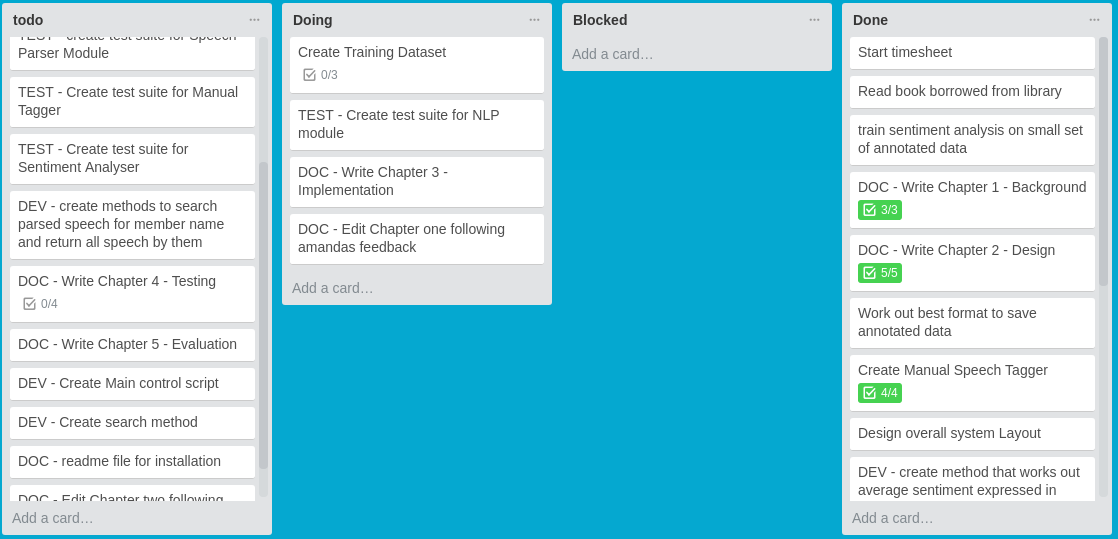
\includegraphics[width=\textwidth]{trello_board_screenshot}
	\caption{Screenshot of a Trello Board showing work in progress, done, and not yet started}
	\label{fig:trello_screenshot}
\end{figure}

In utilizing this tool for the organization of the project, development was planned out. Each "Card" of the board represented one task, and could be moved between columns. More complicated tasks were broken down into separate tasks, or a checklist could be added to a card, should the task need to remain as a single task for whatever reason.

\section{Conclusion}
Now that the background work has been documented, this report will move on to look at the design process of the project, documenting the choices made for each part of the project and the reasoning behind them, and showing some of the design work undertaken.
%\addcontentsline{toc}{chapter}{Development Process}
\chapter{Design}

In FDD, large, detailed design documents are not necessary. A simple overview of desired features and a breakdown of the overall system are sufficient, and are what will be detailed in this chapter.

\section{Overall Architecture}
As the project was developed using Feature Driven Development (FDD), the initial design of the system focused on the desired features of the system. These features were:
\begin{itemize}
	\item Download the dataset.
	\item Parse the original data into a more useful format.
	\item Allow a user to annotate the data with sentiment, to generate training and testing datasets.
	\item Train an AI algorithm on the datasets generated.
	\item Search the parsed data to find speech about a certain topic, or by a particular Member of Parliament.
	\item Use the trained AI algorithm to extract sentiment from the speech found.
	\item Display a comparison of the sentiment expressed about a topic or by an MP over time.
\end{itemize}

Using these features, the overall system can be designed, and an unofficial class diagram can be created that can help guide implementation.

\begin{figure}[ht]
	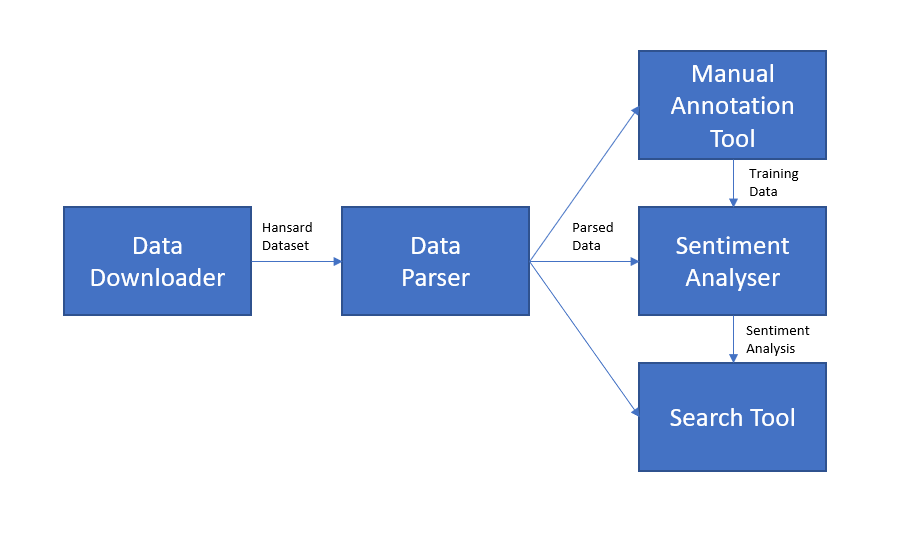
\includegraphics[width=\textwidth]{project_block_diagram}
	\caption{Functional block diagram of the overall system. Arrows represents data movement}
	\label{fig:project_block_diagram}
\end{figure}

As seen in fig.\ref{fig:project_block_diagram}, the system is broken down into functional blocks, each representing a distinct part of the system. They were split this way to maintain readability in the source code. Whilst it would have been possible to keep all functionality in a single file, it would have made maintaining the code very difficult. Each functional block is therefore a separate class in the Python source code, so any interaction between them is easy to manage.

\subsection{Data Downloader}
The Data Downloader is designed to download all of the Hansard Dataset from the site on-line, and store it locally for use by the rest of the system. It is likely that this first block will only need to be run a single time, but still proves useful in ensuring all the data is downloaded.

The files are to be downloaded from the \href{http://www.hansard-archive.parliament.uk}{Hansard Archive} page. Each of the six series has a subdirectory under that root page, that contain all the data files. The data files have a distinct naming pattern that can be referenced using something like Regular Expressions in order to automate the downloading and searching of the files.

Originally, this was not going to be a part of the main system, as it is possible to download the data manually. However, only ten files are displayed on the web page each time, and some of the series have up to a thousand files to download. This can be seen in fig.\ref{fig:Archive_Screenshot}

\begin{figure}[ht]
	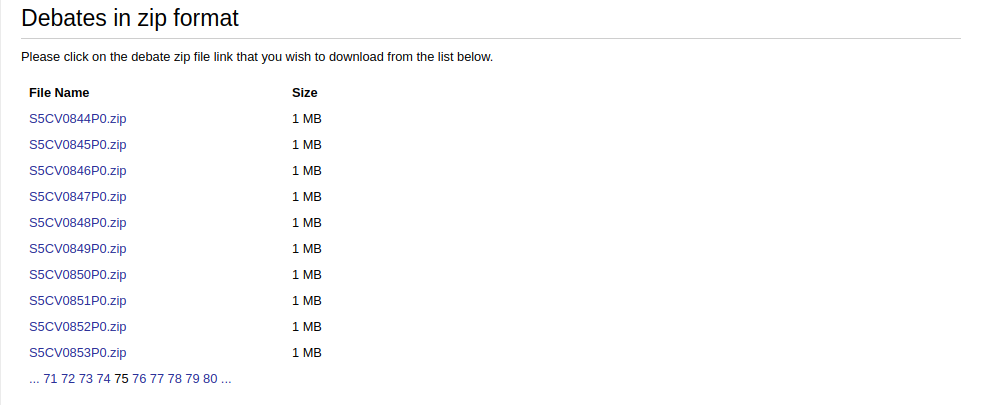
\includegraphics[width=\textwidth]{archive_screenshot}
	\caption{Screen capture from the Hansard Archive website, showing the number of files available}
	\label{fig:Archive_Screenshot}
\end{figure}

\subsection{Data Parser}
The Parser is designed to read the original files downloaded by the Data Downloader, and save all relevant data in separate location, in a more consistent layout than that of the original dataset. This should allow any usage of the data from other parts of the system to be much simpler, and thus faster and less prone to error. It should ensure speech is always attributed to the correct person, even if their names are presented differently. This means the Data Parser will have to utilize a part of NLP known as Name Disambiguation, which is not a simple task. 

\subsection{Manual Annotation Tool}
The Manual Annotation Tool (the MAT) is designed to allow a user to create a testing and training dataset from the parsed data. It should show a selection of speech to the user, and ask them to annotate it as either a positive sentiment, negative sentiment, or neutral sentiment. These choices will be recorded, and can then be used to train a machine learning algorithm to extract sentiment from the remaining data. It would also provide the option to edit the text, the MP's name, or the topic title, to allow the user to correct typos transfered from the original dataset.

Originally, the MAT would display an entire paragraph of speech, displaying everything a Member of Parliament said about a topic on a particular day. However, this would often display too much text, with parts showing positive sentiment and other parts of the same text showing negative sentiment. Additionally it was realized that attempting to train an AI algorithm on these large blocks of text would be far too complex. For those reasons, the MAT was modified so that it would only display a single sentence at a time, allowing a more accurate way of annotating sentiment.

\subsection{Sentiment Analyzer}
The Sentiment Analyzer will use the datasets generated by the MAT and produce a model based off the data. It should also provide the ability to load a previously trained model, rather than spend time retraining every time the system is run. Once trained or loaded, it should be able to accept blocks of text, which it can then extract sentiment from, and return it.

As AI algorithms are trained on "Features" rather than plain text, the Sentiment Analyzer must have some method of converting a sentence or paragraph into a set of features for the algorithm to use. Following on from a tutorial found on Youtube \cite{NLTKYoutubePlaylist}, it appears that a good way to turn the text into a set of features is to use a dictionary, where the keys are the most used words from the training set, and the value is a True or False, for if the word is contained in the sentence or paragraph given. The potential issue with this is the loss of context, as separating the words completely will lose any negation, such as in the sentence "This is not good".

\subsection{Search Tool}
The Search Tool will be used by the user to search through the data for a particular Member of parliament, to get their speech and its sentiment, or for a particular topic, to get the sentiment expressed about that topic. 

\section{Data Design}
As parts of the system were designed to modify the layout of the original data at times, the formatting of said data had to be designed as well.

\subsection{Parsed Data}
For the parser, the format of the data files that it produces was originally designed as thus:
\begin{lstlisting}[language=XML]
<date dateformat="1984/04/13">	
    <speech>
        <member>memberName</member>
        <topic>topicTitle</topic>
        <stance>POS/NEG</stance>
        "Actual Text of Speech would go Here"
    </speech>
    ....
</date>
....
\end{lstlisting}
The ellipses represent repeats, so inside the \emph{Date} tags, multiple \emph{speech} tags, all formatted like the one shown, can exist. A file may also contain multiple \emph{Date} tags. 

This, however, was causing some issues during development based around the size of the produced files, as each entire series of data was being parsed into the same file. In order to combat the slow speeds of accessing such large files, and other issues caused by the layout, the data format was changed. Now, each unique date found within the source had a separate file, and within this file the data was formatted in its final form.
Each date file is an XML file, the structure of which can be represented as a tree, shown in fig.\ref{fig:parsed_data_tree}.

\begin{figure}[ht]
	\includegraphics[width=\textwidth]{parsed_data_tree}
	\caption{Diagram showing the structure of the parsed data, in XML. The \emph{Date} tag is the root of the file}
	\label{fig:parsed_data_tree}
\end{figure}

Each file can contain multiple member tags, which each have the member of parliament’s name as an attribute. Each member tag can contain multiple tags for the topics they discuss, each of which have the topic title as an attribute. Each topic tag can have multiple speech tags, each speech tag containing the verbatim copy of what the member said about the particular topic.

\subsection{Annotated Data}
The formatting of the annotated data files was also designed at this stage. It was decided that the files would be saved as CSV files (comma separated values), which is a simplistic database style where a line in the file represents a single record, each value of the record being separated by a comma, hence the name. The layout was designed as the following:

\textbf{Sentence; Sentiment; Member; Topic}

As shown, it was decided that the best way of annotating full speech was to split it by sentence, so that each sentence would be annotated with its own sentiment. This would simplify the training process for the machine learning algorithms, as it was thought that trying to train it on too large a block of text would result in sub par results.

\section{User Interface}
Due to the complexity of the project, it was decided that the system would only be interacted with via the command line. This meant that, beyond basic menus, no GUI had to be designed for use. It was though that, should there be time during or after the project development, a GUI could be designed which worked by interacting with the command line interface in the background, but it was not considered system critical to have such a thing.

\section{Algorithm Design}

\subsection{AI Algorithm Choice}
There are many potential algorithms that may be chosen for this project. It may prove difficult to choose one, or more, without simply trying them. The design calls for the use of Naive Bayes at first, mainly as its one provided by the NLTK package. However, multiple other algorithms may be tested, and the results compared to decide on the final choice. Should multiple algorithms prove useful, a voting system could be implemented, which applies each algorithm, and they cast a vote to what sentiment they "think" applies. The votes would then be counted and the result shown.

\subparagraph{Naive Bayes}
Naives Bayes is a supervised algorithm with uses the statistical analysis of Bayes Theorem as to classify data. It treats each feature as completely distinct, which isn't accurate for NLP, but will may suffice for development of the system.

\subsection{Parsing}
The Data Parser needs to find and extract useful speech from the original data. Though said data is somewhat disorganized, there are exploitable patterns that the Parser can use to find as much speech as possible. The overall method is documented in the following pseudo-code:
\begin{lstlisting}
FOR EACH FILE
    FOR EACH DATE TAG
    	IF(DATE_FILE FOR DATE EXISTS)
        	LOAD DATE_FILE CONTENTS INTO DATE_XML
    	ELSE
        	CREATE FILE
        	CREATE DATE_XML
    	FOR EACH CONTRIBUTION IN DATE_TAG
        	GET CONTRIBUTION PARENT_TAG
        	GET MEMBER NAME AS CHILD OF PARENT_TAG
        	GET TITLE AS SIBLING OF PARENT_TAG
        	GET SPEECH FROM CONTRIBUTION
        	IF MEMBER HAS BEEN SEEN BEFORE IN CURRENT DATE_FILE
        	    IF TOPIC HAS BEEN DISCUSSED BY MEMBER BEFORE
        			ADD SPEECH TO TOPIC
        		ELSE
        			CREATE NEW TOPIC
        			ADD SPEECH
        	ELSE
        		CREATE NEW MEMBER TAG
        		ADD TOPIC TO MEMBER TAG
        		ADD SPEECH TO TOPIC
        	ADD SPEECH TO DATE_XML

    SAVE XML TO DATE_FILE (OVERWRITE)
\end{lstlisting}

This shows that, so long as the parser can find a tag in the source XML for the date, all other relevant information can be found in relation to the position of this date tag in the XML. It also shows the method of ensuring all speech by one Member of Parliament is correclty attributed to them, to avoid repeated mentions of the same MP in the same file.
%\chapter{Implementation}

%The implementation should look at any issues you encountered as you tried to implement your design. During the work, you might have found that elements of your design were unnecessary or overly complex; perhaps third party libraries were available that simplified some of the functions that you intended to implement. If things were easier in some areas, then how did you adapt your project to take account of your findings?
%
%It is more likely that things were more complex than you first thought. In particular, were there any problems or difficulties that you found during implementation that you had to address? Did such problems simply delay you or were they more significant?

%You can conclude this section by reviewing the end of the implementation stage against the planned requirements. 
	
\section{Data Downloading}
\label{sec:imp_data_download}
%discuss data downloader implementation, discussing file name pattern and challenges with that, as well as %difficulties with storage as dataset is large
One of the first parts of the system to be implemented was the Data Downloader. This was done first in order to get the full dataset downloaded as fast as possible, and also as a form of Python practice.

As mentioned in Section \ref{sec:des_data_downloader}, the files that needed to be downloaded from the online archive had a specific format that made finding all the files required easier. Each series had a specific URL, and all files for that series would be stored as children of that URL in zip files. The naming pattern for the files was as follows:

\textbf{S\emph{s}V\emph{vvvv}P\emph{p}.zip}

where \emph{s} is the series from 1 to 6, \emph{vvvv} is 4 digits representing the volume of the series, starting at 0001, the max value depending on which series it is a part of, and \emph{p} is a part number, as some files were split into multiple parts. This could be zero, if the file is not split, or a one or two if it has been split. For instance, \emph{S6V0141P1.zip} would represent the \emph{1st} part of the \emph{141st} volume in series \emph{6}.

There was one difference to this pattern, discovered during development. Series 5 of Hansard was separated into records for the \emph{House of Commons} and the \emph{House of Lords}. For these, the letter \emph{C} or \emph{L} was added before the V to differentiate the two series. Afterwards, series 6 also contained the letter \emph{C} to show that it was also only for the house of commons. So, for Series 6, volume 141, part 1, the file format would actually be \emph{S6CV0141P1.zip}.

\subsection{Online Connection}
\label{sec:imp_online_connect}
Python has a commonly used library for HTTP connections called \href{http://docs.python-requests.org/en/master/}{\emph{Requests}}. It provides an API (\emph{Application Programming Interface}) allowing easy connection to a provided URL, simply by providing a URL. Using this API, the downloader can check to see if a file exists, using the code snippet Algorithm \ref{lst:downloader_snippet}.

\begin{lstlisting}[float=ht,
				   caption={Snippet of the Downloader Code},
				   label={lst:downloader_snippet}]
for i in range(0, 100):  # change depending on how many files it looks like exist
    for j in range(0, 4):  # just to make sure. Not seen any files with P3 at the end but you never know
        temp_url = '{}{}/{}'.format(url_base, url_add[series-1], file_name_format.format(series, i, j))
        print("Checking: {}".format(file_name_format.format(series, i, j)))
        r = requests.get(temp_url)
        status = r.headers['content-type']
# if the zip file exists, the type will appear like this:
        if status == 'application/zip; charset=utf-8':  
            print("FILE FOUND")
            zip_ref = zipfile.ZipFile(io.BytesIO(r.content))
            zip_ref.extractall(save_loc)  # extract the file
            zip_ref.close()

        else:  # if the zip file doesn't exist an error page is returned instead
            print("FILE NOT FOUND")
\end{lstlisting}

Effectively, this code snippet loops through the files following the described pattern, and gets the status of the constructed URL. the \emph{header} part returns a string that describes the type of file returned, as if the file does not exist, it still returns a 404 error page rather than not returning anything. If the file does exist, however, it returns a string that says it is a ZIP file type (\emph{"application/zip"}).

If the file does exist, the downloader also makes use of a library called \emph{zipfile}, which allows it to handle zip files internally. It can then extract the data file from the compressed zip file, and save it to the designated directory on the local machine.

\subsection{Dataset Size}
\label{sec:imp_dataset_size}

The total Historical Hansard Dataset that was downloaded by the project is \emph{14.4GB}, and consists of \emph{2503} files, demonstrating the need for the automated downloading. Due to this size, the dataset could not be saved to the University file system, and so was saved to an external hard drive instead. This meant that some parts of the later development were slowed due to the USB 3 connection used by said hard drive. 

\section{Data Parsing}
\label{sec:imp_data_parse}
%discuss experimentation with how to extract data from original dataset. discuss change made to format of parsed data part way through to make it easier to annoate.
During development of the system, the Data Parser and associated methods were where the most time was spent, due to many unforeseen complications.
 
\subsection{Name Recognition and Disambiguation}
\label{sec:imp_name_disamb}
%here discuss difficulties in name disambiguation. discuss attempted methods of using NLTKs named entity %thing and the implemented regex solution. Discuss how the regex solution only works because the names are %presented in a predicable pattern, and would not be valid outside of this dataset
Part of the difficulty in parsing the data accurately was ensuring speech spoken by one person was always attributed to that person, even though the references to that person may use multiple versions of their name. In order to correctly attribute speech to the speaker, without duplicating references to them, a method of NLP called "Name Disambiguation" must be employed.

Name Disambiguation is the method of identifying proper names in text, and recognizing when two proper names refer to the same subject or person.\cite{Wacholder1997} Many difficulties exist for such a task, as names can come in many forms. Proper nouns can often refer to multiple things. \emph{Johnson and Sons} might refer to a business by that name; two people with the surnames \emph{Johnson} and \emph{Sons}; or someone called \emph{Johnson} and their male children. In this example, the context of the sentence the name appears in may provide clues to which it is, but this is not always an option.

Thankfully, this project only needs to be able to recognize the names of the Members of Parliament mentioned in the Hansard Dataset, which displays more structure in the way it names people than normal human speech would.

\begin{figure}[ht]

\includegraphics[width=\textwidth]{dataset_name_example}
\caption{An example from the original dataset, showing that names exist only within \emph{member} tags}
\label{fig:dataset_name_example}
\end{figure}

As can be seen in Figure \ref{fig:dataset_name_example}, the names needed for this project are always contained within a \emph{member} tag. They still contain the full job title at times, but this means that the area the project needs to look for a name is well defined. It can be guaranteed that, if a member tag is encountered, it will contain the name of the member.

The first attempted method of extracting the name from the \emph{member} tag was using the \emph{Named Entity Chunker} from NLTK, which is designed to extract the Named Entities from a piece of text and return them in a list. Using this, the name could be extracted, potentially along with other parts of the title (\emph{The Under-Secretary of State for Trade (Mr. Reginald Eyre)} would be returned as a list of two names, \emph{State for Trade} and \emph{Mr. Reginald Eyre}). The thought was that the actual name desired could be chosen from that list by looking for the item that started with an Honorific, such as \emph{Mr.}, \emph{Mrs.} and other such titles. However, the Named Entity Chunker did not work consistently enough for it to be a viable solution for the name extractor, as it often separated the honorific from the name. Due to this, it could not be reliably used to extract the names, because there was no way to recognize, when it returned multiple names, which referred to the actual person, and which was a part of their job title.

The second method attempted, which was the one settled on for the project, was the use of Regular Expressions to search for the expected name format. This method relies on a lot of assumptions about the organization of the original dataset, but appears to be good enough for the current dataset. The assumptions are as follows:
\begin{itemize}
	\item All Names start with an Honorific (Mr, Mrs, Sir etc)
	\item All Names End with a Surname
	\item The first time a person is seen, their full name and job title, if relevant, are presented
\end{itemize}

Following these assumptions, Regular Expressions could be used to find the honorific at the start of the name, then get everything following it until either the end of the text, or a piece of punctuation not commonly used in names, such as a bracket.
\begin{figure}[ht]
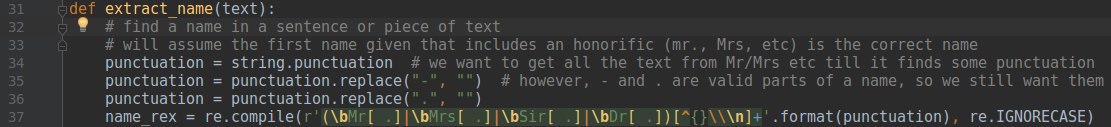
\includegraphics[width=\textwidth]{extract_name_code_example}
\caption{Extract of code from the Name Extractor Method.}
\label{fig:name_extract_code}
\end{figure}

Figure \ref{fig:name_extract_code} shows the regular expression used to extract a name from a piece of text. It searches for an Honorific to start it off, either \emph{Mr}, \emph{Mrs}, \emph{Dr} or \emph{Sir}. Once it finds one of these honorifics it gets everything after it that is not a punctuation mark listed, as shown by the \verb|[^{}\\\n]+| part at the end of the regular expression. The \verb|{}| brackets in that part are replaced with the string called \emph{punctuation}, generated by the string package, so that it becomes a list of all punctuation possible, including new line characters.  

\subsection{Name Matching}
\label{sec:imp_name_match}
Once names can be reliably extracted from the source text, a method of comparing two names to see if they referred to the same person had to be developed. This becomes a very complicated issue, simplified only slightly by the assumptions mentioned previously.

\begin{table}[ht!]
\centering
\begin{tabular}{|c c c|}
Name One & Name Two & Same Person? \\
\hline
Mr. Adam Neaves  & Mr. Adam Neaves & True \\
Mr. A. Neaves    & Mr. Adam Neaves & True \\
Dr. Adam Neaves  & Mr. Adam Neaves & False, wrong Honorific \\
Mr. B. Neaves    & Mr. Adam Neaves & False, wrong First Name \\
Adam Neaves      & Mr. Adam Neaves & True, despite missing honorific \\
Mr. A. B. Neaves & Mr. Adam Neaves & True, though slightly ambiguous \\
Mr. A. B. Neaves & Mr. Neaves      & True, though again ambiguous    \\
\end{tabular}
\caption{Table showing the different ways names might or might not refer to the same person}
\label{tbl:name_match}
\end{table}

For instance, as shown in Table \ref{tbl:name_match}, first names might be shortened to just an initial, or even fully removed. Honorifics are not guaranteed to be present, but are very important if they are, as two different names may differ from only that.

The implemented algorithm for this project follows the same assumptions mentioned in Section \ref{sec:imp_name_disamb}, and is designed to allow for some false negatives (wherein two names that \emph{do} refer to the same person might not appear as the same person) to avoid any false positives at all. This is because it was decided that speech accidentally attributed to the wrong person would be worse than accidentally having duplicate references to a person, since a human reader can likely see the connection between \emph{Mr. Adam Neaves} and \emph{Mr. A Neaves}, but there would be no way for them to know that some speech was attributed to the wrong person. The basic algorithm implemented is as shown in Algorithm \ref{lst:name_match}.
\begin{lstlisting}[float=ht,
				   caption={Pseudocode representing the name matching method},
				   label={lst:name_match}]
if BOTH NAMES ARE EXACTLY THE SAME
	return True
SPLIT BOTH NAMES INTO COMPONENT WORDS
for EACH NAME
	if NAME CONTAINS 3 WORDS
		FIRST WORD IS HONORIFIC
		SECOND WORD IS FORENAME
		THIRD WORD IS SURNAME
	else
		FIRST WORD IS HONORIFIC
		LAST WORD IS SURNAME
		IGNORE ANYTHING ELSE
if FORENAME ONE and FORENAME TWO BOTH EXIST
	FORNAME_MATCH = FORNAME ONE == FORNAME TWO
else
	FORNAME_MATCH = True
SURNAME_MATCH = SURNAME ONE == SURNAME TWO
HONORIFIC_MATCH = HONORIFC ONE == HONORIFIC TWO

if SURNAME_MATCH, HONORIFIC_MATCH and FORENAME_MATCH ARE True
	return true
else return False
\end{lstlisting}

This method does work so long as the assumptions in Section \ref{sec:imp_name_disamb} hold true. It would not be a valid method of matching names in a more generalized setting where the formatting and appearance of names would vary wildly.

\subsection{Saving Parsed Data}
\label{sec:imp_saving_pased_data}

The parser would save the information extracted from the original data files in newly created XML files. Due to some character use in the original dataset, these files had to be opened by the Python script in \emph{Binary Mode}, meaning it would treat the data as bytes of data rather than strings of text. Due to this, when editing a file, the Parser could not simply append data to the file, but rather would have to overwrite the whole file. Therefore, when editing a parsed file to add more data to it, it was necessary to load the whole file into memory, edit that data, then overwrite the whole set of data to the XML file again.
This was one of the main reasons for the change in data structure part way through implementation described in Section \ref{sec:des_parsed_data}. When the Parser was designed to write an entire series to a single file, it would take an increasingly long time to read the whole file into memory, then save the data back to the file once modified. At the start of a session of parsing, it would take an average of \emph{3 seconds} to parse the first file from the original dataset, but as it parsed more of a series, each additional file would increase the time it took substantially. Table \ref{tbl:original_parse_time} shows the time taken on a subset of one series.

\begin{table}[ht!]
\centering
\begin{tabular}{c | c}
	\textbf{Source Data File Number} & \textbf{Time to Parse (s)} \\
	\hline
	0001 & 2.564   \\
	0002 & 3.245   \\
	0003 & 4.632   \\
	...  & ...     \\
	0250 & 302.452 \\
	0251 & 306.321 \\

\end{tabular}
\caption{Excerpt from the log of the original parser parsing Series 6, showing time it took to parse each file}
\label{tbl:original_parse_time}
\end{table}

As can be seen, the additional time taken for each file meant that, in order to parse an entire series, the parser would take up to a few hours to finish. Additionally, as the large files had to be loaded into memory in order for them to be edited, the Parser would use a large amount of RAM, at one point during development getting up to around 10GB of RAM used.

Therefore, instead of saving an entire series worth of data to a single file, the decision was made to split the files by date instead. The parser would search through each file, creating a new file for each date it encountered, so that everything that was debated on that date would be saved to that file. This meant that the parsed data files were smaller, and meant that the data that had to be loaded into memory in order to be modified was much smaller, so the Parser didn't use anywhere near as much RAM. It also meant that the time taken per file parsed was constant, and only depended on the size of the original file, rather than the number of files already parsed. This was a much better solution, and also encouraged a better design for the parsed data layout, as described in Section \ref{sec:des_parsed_data}.

Additionally, though the parsed data consisted of more files than the original dataset, the set of parsed data was usually smaller than the original, due to the parser stripping out unneeded information. The exact values can be seen in Table \ref{tbl:parsed_data_size_comp}

\begin{table}[ht!]
\centering
\begin{tabular}{r || l | l || l | l}
	& \multicolumn{2}{|c||}{\textbf{Original Dataset}} & \multicolumn{2}{|c}{\textbf{Parsed Dataset}}\\
	\hline
	\textbf{Series} & \textbf{Size (GB)} & \textbf{Number Of Files} & \textbf{Size (GB)} & \textbf{Number Of Files}\\
	\hline
	\hline
	1 & 0.0943 & 27   & 0.0691 & 1245\\
	2 & 0.0877 & 22   & 0.0755 & 926\\
	3 & 1.4    & 305  & 1.2    & 6888\\
	4 & 0.6461 & 133  & 0.3842 & 1551\\
	5 & 5.5    & 900  & 3.4    & 9742\\
	6 & 3.5    & 446  & 1.7    & 3745\\
\end{tabular}
\caption{Size comparison between the Original Hansard Dataset and the Parsed Dataset generated by the Parser}
\label{tbl:parsed_data_size_comp}
\end{table}

\section{Manual Annotation Tool}
\label{sec:imp_manual_annotate}

With all the source data successfully parsed, the Manual Annotation Tool (MAT) could be developed to use that data to create the training dataset discussed in Section \ref{sec:des_anotate_data}.

Originally, as discussed in Section \ref{sec:des_annotation_tool}, this tool was designed to print everything a single MP said about a particular topic, but this often meant far too much text was printed on the screen at any one time. Additionally, this tool was also designed to allow the user to edit the name of the MP, or the topic, in case of typos in the text. However, it was felt that the tool was overcomplicated by this added functionality.

Instead, the Annotation tool now only displays one sentence at a time, and allows the user to quickly annotate it by entering only a single character, as shown in Figure \ref{fig:annotate_screenshot}. That helped to speed up the process of annotating data, which was already a lengthy process, in order to create the training set needed for the Artificial Intelligence Algorithm.

\begin{figure}[ht]
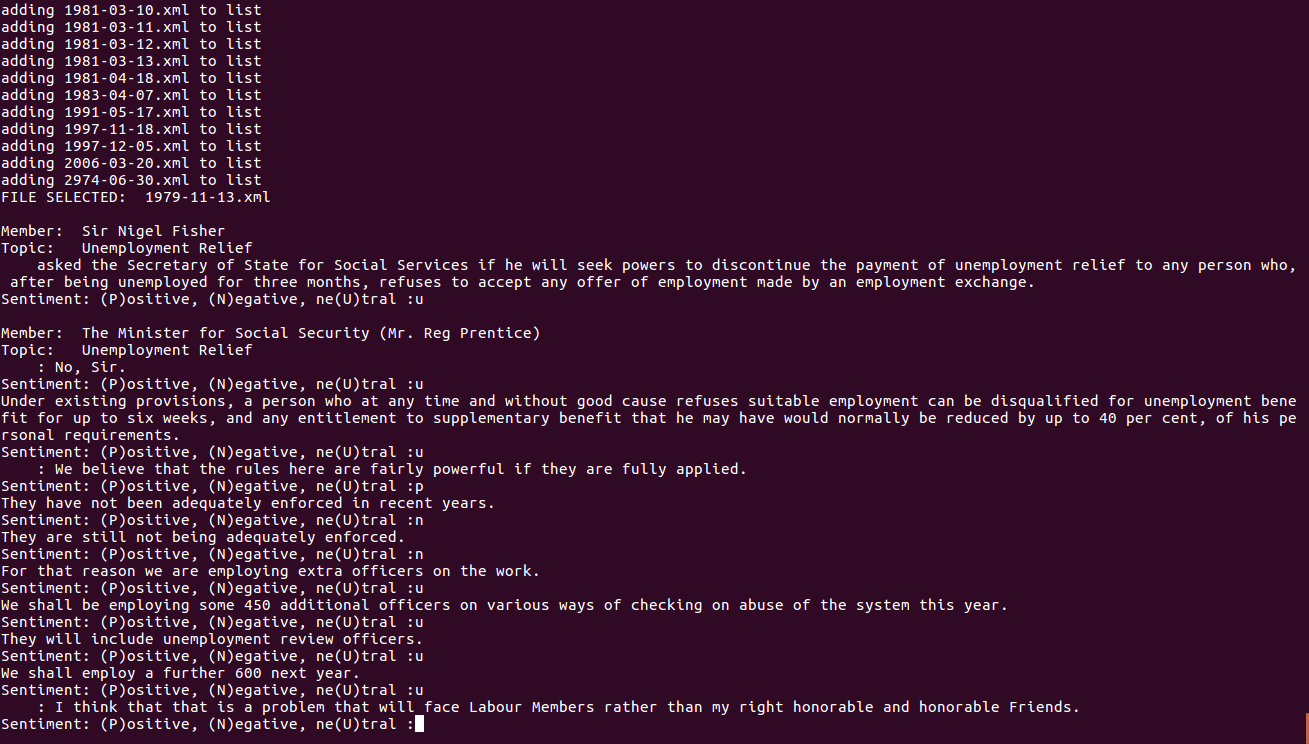
\includegraphics[width=\textwidth]{annotate_screenshot}
\caption{Screenshot from the Annotation Tool running on the Command Line}
\label{fig:annotate_screenshot}
\end{figure}

\subsection{Sentence Splitting}
\label{sec:imp_sentence_split}
% discuss dificulties getting NLTKs sentence tokenizer to work with the data
An important part of the update to the Annotation tool was the ability to separate a block of text by sentence. This is not as simple as it sounds, as the text can't just be split whenever a \emph{"."} character is encountered, as there are acronyms in some of the text, and some sentences might include a quote with a period in it, which must be included in the sentence structure.

NLTK does include a sentence tokenizer as a part of its library. This method is designed to receive a block of text as an input, and returns an array of sentences, split by the tokenizer. However, this function did not work perfectly for the data used, as there were a few special cases, such as typos, that the tokenizer provided was not prepared for. In order to improve the quality of the splitting, some parts of the text had to be modified, so that the tokenizer would either stop seeing sentence boundaries where there were none, or missing sentence boundaries. These changes were as follows:

\begin{itemize}
	\item The word \emph{Honourable} had to replace the word \emph{Hon.}, which was often used as a short hand. NLTK's tokenizer did not recognise this and therefore split sentences on the period of that word.
	\item If the Members of Parliament discussed some form of percentage, it was commonly referred to as \emph{per cent.}, which the sentence tokenizer saw as the end of a sentence due to the period. This was replaced with the word \emph{percent}.
	\item The Parser would strip out any new line characters from text before saving it. This, combined with issues from the original data, meant that when a sentence ended, it was common for it to miss out any sort of space between the period that marked the end of the sentence, and the start of the next sentence. Due to this missing space, the tokenizer wouldn't realize that it was supposed to be a sentence boundary and therefore wouldn't split the text. Regular expressions were used to find areas of text where it looked like this had occurred, and would input the space.
\end{itemize}
 
Following these corrections, the code that performed the sentence splitting became that shown in Algorithm \ref{lst:sentence_split}.

\begin{lstlisting}[float=ht,
				   caption={Sentence Splitting method, with included regular expressions},
				   label={lst:sentence_split}]
def sentence_split(text):
	# because NLTK's sentence tokenizer recognises hon.
	# as the end of a sentence, unlike mr. or mrs., we need to
    # replace that with something it can handle    
    regex_hon = re.compile(r'\bhon\.', re.IGNORECASE)
    regex_percent = re.compile(r'\bper cent\.', re.IGNORECASE)
    # some sentences are missing the space. Add it back in.
    regex_sentence_end = re.compile(r'([a-z])\.([A-Z])') 
    text = re.sub(regex_hon, "honorable", text)
    text = re.sub(regex_percent, "percent", text)
    text = re.sub(regex_sentence_end, r'\1. \2', text)
    text = text.replace('\n', ' ')
    # once all regex is done, send text to the tokenizer
    return sent_tokenize(text)
\end{lstlisting}

As can be seen by this function, each replacement required is handled using regular expressions, which allow it to quickly search the whole text given to it for these issues described, and fix them, before the text is then sent to the sentence tokenizer of NLTK to be split into an array. This method works well, though it is not the most maintainable, as it would have an issue if many more special cases were found.

\section{Sentiment Analyser}
\label{sec:imp_sentiment_analyzer}

The sentiment analysis tool builds upon the methods provided by NLTK. The tool provides a method to train the AI algorithm, and also methods to analyze the sentiment for sentences and paragraphs using the trained algorithm. Though NLTK does provide a sentiment analyser as part of its package, this was a pre-trained algorithm that had been trained on a Movie Review corpus. It was therefore expected that such an algorithm would not be suitable for this project, as no way to retrain on custom data was found. Therefore, a custom sentiment analyser was created using the Naive Bayes Algorithm.

This Sentiment Analyser was first trained on only a small set of training data designed only to be enough to allow development. Without a small dataset, the Sentiment Analyser module could not be developed, as there would be no way of testing that it functioned without anything to base the AI model on.
% discuss issues with not annotating enough data.
\subsection{Naive Bayes Classifier}
\label{sec:imp_naive_bayes}
% discuss results of Naive Bayes. Discuss choice of features (top 3000 most popular words, true of false)

Naive Bayes, as described in Section \ref{sec:des_naive_bayes}, was the AI algorithm provided as a part of the NLTK library.

\subsubsection{Creating Features}
\label{sec:imp_create_features}

Features, in the case of AI training, are a representation of the thing an AI is trying to learn to predict\cite{Mitchell1997}. For instance, if an AI algorithm was being trained to predict the weather based off current conditions, the current conditions would be the set of features, each separate condition such as  current temperature, barometric pressure, humidity etc. would be a feature. In the case of a supervised algorithm, such as Naive Bayes, it is provided with a list of features, and the class that is attributed to that set of features. So, for the example given, Table \ref{tbl:weather_feature} would be an example set of training data.

\begin{table}[ht!]
\centering
\begin{tabular}{r | r | r || l}
\textbf{Temperature} & \textbf{Pressure} & \textbf{Humidity} & \textbf{Weather Class} \\
\hline
Low  & Medium  & High & \textbf{Storm}    \\
High & Low     & Low  & \textbf{Sunshine} \\
High & Low     & High & \textbf{Storm}

\end{tabular}
\caption{Weather training data as an example of features}
\label{tbl:weather_feature}
\end{table}

In order to be able to use the training data to train the algorithm, the data must first be turned into a set of \emph{Features} that the algorithm could use to base its hypothesis on. Following the Tutorial by \textbf{Sentdex}\cite{NLTKYoutubePlaylist}, it was decided that the feature set would be the set of 3000 most commonly used words from the training dataset, after removing \emph{Stop Words}, which are words too common in the English language to be of any use to the classifier, such as \emph{The}, \emph{for}, or \emph{to}. The set of features would be represented by a \emph{Key Value dictionary}, where the word acts as the unique key for each value, and the value is a Boolean, representing whether or not the word is present in the text. This method has its limitations, discussed in Section \ref{sec:evl_AI}. However, it does limit the effect of uncommonly used words, as they won't be a part of the feature set and can therefore be ignored by the algorithm.

\subsubsection{Training the Algorithm}
\label{sec:imp_train_algorithm}
To train the algorithm, the set of features created is first split into a set of training data, and a set of testing data. The algorithm is trained on the training data, using the combination of features and annotated classes, then it classifies the testing data using the hypothesis generated by the training. The accuracy of the algorithm is then represented as the percentage of these training cases correctly classified.

For this project, the set of annotated features was shuffled, so that they would be in a random order, in an attempt to reduce the changes of bias. It then, in the original iteration of the project, split the set of feature/annotation pairs so that the first 90\% were the training data, and the remaining 0\% were the testing set. This, however, often gave very mixed results, in part due to the randomization, as the resulting AI model would have a claimed accuracy of anywhere between 40\% and 90\%.

Instead, it was decided to use \emph{K-Fold Cross Validation}\cite{Hastie2009}, in which the set of annotated features was split into \emph{K} chunks. For each chunk, the algorithm was trained on the rest of the data, and tested on the single chunk, as shown in the diagram of Figure \ref{fig:k_fold_diagram}. It was then trained on the entire set of features, the model from such training was the one used and saved.

\begin{figure}[ht]
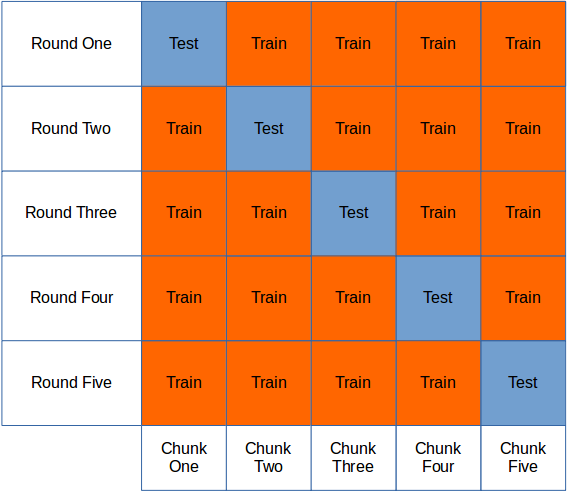
\includegraphics[width=\textwidth]{k_fold_diagram}
\caption{Diagram showing how K-fold validation works, when $k=5$. Rows represent training rounds, columns are the chunks of data.}
\label{fig:k_fold_diagram}
\end{figure}

The partitioning of the data was done after the feature list was shuffled to ensure the chunks were random. The code that trained and tested the model is in Algorithm \ref{lst:train_AI}. the variable \emph{fold} is the number of folds to make, and the variable \emph{features} is the list of annotated features, having been randomly shuffled.

\begin{lstlisting}[float=ht,
				   numbers=left,
				   caption={Snippet of code that trains and tests the classification algorithm},
				   label={lst:train_AI}]

print("Splitting feature set into {} folds".format(fold))
folds = numpy.array_split(features, fold)  # split into folds for training
# for each fold, train it on all other folds, test it on this fold
for i, test_fold in enumerate(folds):
    train_folds = folds[0:i] + folds[i+1:fold]
    train_folds = [item for sublist in train_folds for item in sublist] # flatten list
    print("Fold {}. Training on {} Instances.".format(i+1, len(train_folds)))
    classifier = NaiveBayesClassifier.train(train_folds)
    print("Fold Accuracy: {}%".format(nltk.classify.accuracy(classifier, test_fold)))
\end{lstlisting}

\subsubsection{Testing Results}
\label{sec:imp_AI_test_result}

The algorithm was trained and tested using both \emph{10-fold} and \emph{5-fold} validation. Table \ref{tbl:naive_bayes_results_5} and \ref{tbl:naive_bayes_results_10} show the results from this training and testing. The total number of annotated sentences was 201.
\begin{table}[ht]
\centering
\begin{tabular}{r | l | l}
\textbf{Fold Number} & \textbf{Training set Size} & \textbf{Reported Accuracy (\%)} \\
\hline
1  & 160 & 85.366 \\
2  & 161 & 65 \\
3  & 161 & 72.5 \\
4  & 161 & 65 \\
5  & 161 & 67.5 \\

\end{tabular}
\caption{Table of results from training the Naive Bayes algorithm using 10-fold cross validation.}
\label{tbl:naive_bayes_results_5}
\end{table} 

\begin{table}[ht]
\centering
\begin{tabular}{r | l | l}
\textbf{Fold Number} & \textbf{Training set Size} & \textbf{Reported Accuracy (\%)} \\
\hline
1  & 180 & 66.666 \\
2  & 181 & 75 \\
3  & 181 & 85 \\
4  & 181 & 70 \\
5  & 181 & 65 \\
6  & 181 & 60 \\
7  & 181 & 70 \\
8  & 181 & 60 \\
9  & 181 & 80 \\
10 & 181 & 70 \\

\end{tabular}
\caption{Table of results from training the Naive Bayes algorithm using 10-fold cross validation.}
\label{tbl:naive_bayes_results_10}
\end{table} 

As can be seen by these tables, the average accuracy when trained using 5-fold validation was \emph{71.1\%} and when using 10-fold validation it was \emph{70.1\%}. The similarities might well be due to the small number of annotated sentences that were used in training. The problems that caused this are discussed in Section \ref{sec:evl_annotate_data}.

To compare the results, a baseline called \emph{ZeroR}\cite{ZeroR2016} was used. This was used instead of a baseline of random guessing, as it takes into account potential bias in the annotated data. Effectively, \emph{ZeroR} classifies all instances as the most common class, hence the name \emph{Zero Rule}. In the annotated data used, \emph{106} of the sentences are classified as Positive, and \emph{95} are classified as Negative. This means that ZeroR classified all of the instances as Positive, as that is the class with the most instances. The maths of working out the probability of random guessing is shown in Figure \ref{fig:random_prob}, showing that random guessing gives a theoretical accuracy of \textbf{50.1\%}, whereas the Zero Rule baseline has an accuracy of \textbf{52.7\%}. Whilst this difference might not be a large one, it helps improve the analysis of the Naive Bayes algorithm.

\begin{figure}[ht]
$$(P(Class Is Positive)*P(Class As Positive))+(P(Class Is Negative)*P(Class As Negative)) $$
$$(0.527*0.527)+(0.473*0.473)$$
$$0.501$$
\caption{Probability of correct classification based on random selection. $P(X)$ is the Probability of X}
\label{fig:random_prob}
\end{figure}


\subsubsection{Saving the Model}

In order to be useful, the algorithm could not be retrained every time. As the training dataset grows, the time taken to train the algorithm also grows, so it would be inefficient to retrain each time. Thankfully, a python module called \href{https://docs.python.org/3/library/pickle.html}{Pickle} allows for the saving of Python classes as a file on the computer. This module can allow the trained model to be saved and loaded from a file created by the pickle module, and avoids the need to retrain it each time the software is run.

\section{Implementation Conclusion}

Moving on from implementation, this report will now move on to discuss the methods of testing used during and after development, as well as discussing any areas where more rigorous testing, or just more testing in general, would have been useful.
%\chapter{Testing}

%Detailed descriptions of every test case are definitely not what is required here. What is important is to show that you adopted a sensible strategy that was, in principle, capable of testing the system adequately even if you did not have the time to test the system fully.

%Provide information in the body of your report and the appendix to explain the testing that has been performed. How does this testing address the requirements and design for the project?

%How comprehensive is the testing within the constraints of the project?  Are you testing the normal working behaviour? Are you testing the exceptional behaviour, e.g. error conditions? Are you testing security issues if they are relevant for your project? 

%Have you tested your system on ``real users''? For example, if your system is supposed to solve a problem for a business, then it would be appropriate to present your approach to involve the users in the testing process and to record the results that you obtained. Depending on the level of detail, it is likely that you would put any detailed results in an appendix.

%The following sections indicate some areas you might include. Other sections may be more appropriate to your project. 

\section{Overall Approach to Testing}


\subsection{Unit Tests}
%\chapter{Evaluation}
\section{Requirements Comparison}
\label{sec:evl_require_comp}
Table \ref{tbl:requirements_comp} shows the comparison between what required features were set out in Section \ref{sec:des_Architecture}, and what features made it in to the developed system.

\begin{table}[ht!]
\centering
\begin{tabular}{R || L | l | L}
	\textbf{Feature Num} & \textbf{Required Function} & \textbf{Developed Function} & \textbf{Notes} \\
	\hline \hline
	1 & Download the Dataset               & Fully Developed     & \\
	2 & Parse the Original data            & Fully Developed     & Was far more work than anticipated\\
	3 & Provide Ability to Annotate        & Fully Developed     & \\
	4 & Train AI on Annotated Data         & Fully Developed     & Had not annotated enough data \\
	5 & Search parsed data for MP or Topic & Not Developed       & \\
	6 & Use AI to extract Sentiment        & Partially Developed & Only uses naive bayes\\
	7 & Display comparison of sentiment    & Not Developed       & \\ 	
\end{tabular}
\caption{Comparison between required functions and the functions that were developed}
\label{tbl:requirements_comp}
\end{table}

As shown, the project did not manage to complete every requirement that was set out. However, this project did manage to develop an automated sentiment tool that could be trained on the Hansard records, then extract sentiment from sentences or paragraphs given to it, which was one of the main aims of the project.

\subsection{Data Parser Difficulties}
\label{sec:evl_data_parser}

One part of the project that was a much larger part of development than expected was the Data Parser, the development of which is described in Section \ref{sec:imp_data_parse}. As described in that section, parsing the dataset turned out to be a much more complex job than anticipated. Some difficulties came from a lack of prior knowledge on Natural Language Processing. It wasn't realised until a good part way through the development of the parser that Name Disambiguation, discussed in section \ref{sec:imp_name_disamb} was such a complex topic of research, or that it would be such a crucial part of the parsing process. Due to the unexpected complexities of developing the parser, other parts of the project suffered. The \emph{Search Tool} and the \emph{Comparison Tool} were never developed, as the time planned for the development of those modules was instead spent on the Parsing Tool. Additionally, trying to understand the layout of the original Hansard Dataset, especially the earlier series, took a lot of time in the beginning of the project, due to a lack of formatting. Attempting to visualise the large and complex XML files caused a delay in the development of the Data Parser, as there was no way to develop the parser until the data structure was understood.

However, despite these difficulties, once they were overcome the Parser itself works very well. It can accurately pull the relevant speech out of any of the Historical Hansard data files provided, and parse it into files that are much easier to handle. The Name Disambiguation and matching functions, discussed in Section \ref{sec:imp_name_disamb} and \ref{sec:imp_name_match}, might not work for more general name matching, but are tailored towards the Hansard data, and work very well for the project itself.

\subsection{Annotating Data}
\label{sec:evl_annotate_data}

It was expected at the beginning of the project that a large amount of time would have to be devoted to annotating data to train the AI algorithm that would be used. The tool developed, discussed in Section \ref{sec:imp_manual_annotate}, was designed to make this job as easy as possible. However, despite attempts, it still took a large amount of time to annotate any data. Part of the problem is likely as the tool discards any sentences labeled as \emph{Neutral}, since it was thought training on neutral data would not help the task at hand. However, A large part of the speech by Members of Parliament is neutral, when they are either stating facts, or just speaking neutrally. This meant that, if the tool was used to check through 100 sentences to annotate, up to around 40 of those sentences might be neutral, and thus discarded. This means that the training and testing dataset is too small to accurately train the AI algorithm. The tool itself is fully functional and works well for the purpose but, due to time constraints caused in part by the difficulties mentioned in Section \ref{sec:evl_data_parser}, not enough data was annotated, and therefore the performance of the Sentiment Analyser suffered.

There is also a potential for bias in the data annotated. It's possible that, as the data was only annotated by a single person, that there could be some bias in what was claimed to be \emph{Positive}, \emph{Negative} or \emph{Neutral}. It's possible that what was annotated as a \emph{Negative} sentence, for instance, might have only been read as negative by the individual, and not actually spoken in a negative manner. This is partially an issue with written text, as it loses any nonverbal communication, such as body language, which is considered an important part of communication\cite{Whaley2007}.

\subsubsection{Outsourcing Data Annotation}

It was realised too late into the project that there was not enough data, nor enough time to fix the issue. However, there are solutions available that could have prevented this issue. Should this project be restarted, a good idea would be to outsource the data annotation to other people. This would require ethics forms to be filled for every participant, but it would solve the issue of there not being enough time to annotate the data. It would also potentially solve the issue of bias in the annotations, if multiple people were given the same sentence the annotate. This does mean there would be a chance of conflict, if there are multiple different opinions on the sentiment of a single sentence, but these could be solved manually if needed, or automatically in the case of a single person having a different opinion than the rest. This would require more work to combine annotations from multiple sources, but it would replace the time spent doing the annotation without outsourcing.

\subsection{AI Algorithms}
\label{sec:evl_AI}
For this project, the only AI algorithm used was Naive Bayes, as discussed in Section \ref{sec:imp_sentiment_analyzer}. As no other algorithms were tested, it's possible that Naive Bayes may not be the most useful algorithm for this project. Without other algorithms to compare it to there is no way to know. This issue, combined with the small training dataset, means that the Naive Bayes is inconsistent in its accuracy, as shown in Section \ref{sec:imp_naive_bayes}.

\section{Future Work}

If more time could be spent on the project, the following sections discuss what could be done to improve it.

\subsection{More AI Algorithms}

A good use of this additional time would be to implement more than just the one algorithm, and compare results. Should one algorithm prove better than all others, that one should be the one used for this project. If multiple have good results, a voting system could be implemented that ran the multiple algorithms, collected their results, and combined them to form one "voted for" class for the data provided to them. This would require experimentation to check for accuracy and the best method for voting, but could potentially improve the consistency of the results, if not the accuracy.

\subsection{Develop Search Tool}

One of the major failing during development was that the proposed tool designed to search the parsed data for either a Member of Parliament by name, or a topic up for debate, was never developed. While the main aim of the project, to provide a way to train and use an AI algorithm to automatically extract sentiment from political speech, was completed, the use of this is less intuitive without a method to search the pre-existing data for sentiment. Therefore, it could be wise to use any additional time to complete this original project goal.

\subsection{Work with Additional Data Sources}

An interesting fact about the Hansard Report is the number of different forms it is offered in. The one used by the project is the Historical Hansard Dataset, as discussed in Section \ref{sec:bck_hansard}. However, one potential use for this project is to monitor the sentiment expressed by the politicians of today. Hansard is offered in a Daily format, where a report is released in the morning that documents the debates of the prior day. Modifying the Data Parser so that it may also parse these daily reports would give the project a lot more data to work with. Additionally, the Parlimentary website offers an Atom Feed for these reports, which could potentially be subscribed to by the project, so that when a Daily report is released, the parser could automatically download and parse this report, ready to be analyzed by the rest of the system.

\section{Project Conclusion}

A great deal was learned from doing this project, especially from research done into Natural Language processing, and the development of a full project in Python. It is hoped that work can continue on this project after it has been submitted for the dissertation, and may eventually become a useful program for extracting sentiment from political speech.
% add any additional chapters here

\setemptyheader
\addcontentsline{toc}{chapter}{Appendices}
\chapter*{Appendices}
The appendices are for additional content that is useful to support the discussion in the report. It is material that is not necessarily needed in the body of the report, but its inclusion in the appendices makes it easy to access. 

For example, if you have developed a Design Specification document as part of a plan-driven approach for the project, then it would be appropriate to include that document as an appendix. In the body of your report you would highlight the most interesting aspects of the design, referring your reader to the full specification for further detail.

If you have taken an agile approach to developing the project, then you may be less likely to have developed a full requirements specification. Perhaps you use stories to keep track of the functionality and the 'future conversations'. It might not be relevant to include all of those in the body of your report. Instead, you might include those in an appendix. 

There is a balance to be struck between what is relevant to include in the body of your report and whether additional supporting evidence is appropriate in the appendices. Speak to your supervisor or the module coordinator if you have questions about this.

\pagebreak

% start the appendix - sets up different numbering
\fancypagestyle{plain}{%
%\fancyhf{} % clear all header and footer fields
\fancyhead[L]{\textsl{Appendix\ \thechapter}}
\fancyhead[R]{\textsl{\leftmark}}}

\appendix
\fancyhead[L]{\textsl{Appendix\ \thechapter}}
\fancyhead[R]{\textsl{\leftmark}}
\fancyhead[C]{}
\fancyfoot[C]{\thepage}
\renewcommand{\headrulewidth}{0.4pt}
\renewcommand{\chaptermark}[1]{\markboth{#1}{}}

\fancyhead[L]{\textsl{Appendix\ \thechapter}}
\fancyhead[R]{\textsl{\leftmark}}
\fancyfoot[C]{{\thepage} of \pageref{LastPage}}

% include any appendices here
%\chapter{Third-Party Code and Libraries}

If you have made use of any third party code or software libraries, i.e. any code that you have not designed and written yourself, then you must include this appendix. 

As has been said in lectures, it is acceptable and likely that you will make use of third-party code and software libraries. If third party code or libraries are used, your work will build on that to produce notable new work. The key requirement is that we understand what is your original work and what work is based on that of other people. 

Therefore, you need to clearly state what you have used and where the original material can be found. Also, if you have made any changes to the original versions, you must explain what you have changed. 

As an example, you might include a definition such as: 

Apache POI library - The project has been used to read and write Microsoft Excel files (XLS) as part of the interaction with the client's existing system for processing data. Version 3.10-FINAL was used. The library is open source and it is available from the Apache Software Foundation 
\cite{apache_poi}. The library is released using the Apache License 
\cite{apache_license}. This library was used without modification. 
%\chapter{Ethics Submission}

The Ethics form submitted for this project

\includepdf{Appendixes/Ethics_doc.pdf}

%\chapter{Code Examples}

For some projects, it might be relevant to include some code extracts in an appendix. You are not expected to put all of your code here - the correct place for all of your code is in the technical submission that is made in addition to the Final Report. However, if there are some notable aspects of the code that you discuss, including that in an appendix might be useful to make it easier for your readers to access. 

As a general guide, if you are discussing short extracts of code then you are advised to include such code in the body of the report. If there is a longer extract that is relevant, then you might include it as shown in the following section. 

Only include code in the appendix if that code is discussed and referred to in the body of the report. 


\fancypagestyle{plain}{%
   \fancyhead{} %[C]{Annotated Bibliography}
   \fancyfoot[C]{{\thepage} of \pageref{LastPage}} % except the center
   \renewcommand{\headrulewidth}{0pt}
   \renewcommand{\footrulewidth}{0pt}
}

\setemptyheader

\nocite{*} % include everything from the bibliography, irrespective of whether it has been referenced.

% the following line is included so that the bibliography is also shown in the table of contents. There is the possibility that this is added to the previous page for the bibliography. To address this, a newline is added so that it appears on the first page for the bibliography. 
\addcontentsline{toc}{chapter}{Annotated Bibliography} % Adds References to contents page

%
% example of including an annotated bibliography. The current style is an author date one. If you want to change, comment out the line and uncomment the subsequent line. You should also modify the packages included at the top (see the notes earlier in the file) and then trash your aux files and re-run. 
%\bibliographystyle{authordate2annot}
\bibliographystyle{IEEEannotU}
\renewcommand{\bibname}{Annotated Bibliography} 

\bibliography{References/references} % References file

\end{document}